\documentclass[a4paper, 11pt]{article}

% Nécessaire
\usepackage[utf8]{inputenc}
\usepackage[T1]{fontenc}
\usepackage{lmodern}

% Biblio
\usepackage{natbib}
\bibliographystyle{abbrvnat}
\usepackage{hypernat}
\bibpunct{\textcolor{blue}{[}}{\textcolor{blue}{]}}{}{a}{\textcolor{blue}{,}}{;}

\usepackage[french]{babel}
\usepackage{amsmath, amsthm}
\usepackage{amsfonts,amssymb}

% Marge
\usepackage{geometry}
\geometry{margin={2.2cm ,2cm}}

% Figures, graphiques
\usepackage{graphicx}
\usepackage{epsfig}
\usepackage{caption}

% Surlignage
\usepackage{alltt}

\usepackage{xcolor}
\usepackage{soul}
\usepackage{color}
\usepackage{colortbl}

% Indicatrice
\usepackage{dsfont}

\usepackage{multirow}
\usepackage{eurosym}
\usepackage{extarrows}
\usepackage[colorlinks=true, citecolor=blue, linkcolor=.]{hyperref}

% Graphique
\usepackage{tikz}


% Titre
\title{Jeudi}
\author{}
\date{}



\begin{document}
 \maketitle 
 
 On s'intéresse dans ce document aux différents résultats que peut donner le modèle lorsqu'on change certaines hypothèses.
 En particulier lorsque l'on modifie l'arrivée d'individus exogènes ou lorsque l'on introduit un paramètre de «saisonnalité».
 
 \paragraph{Bien ajusté, plein d'exogènes}
 
 \begin{center}
\begin{tabular}{lllllll}
$\gamma$ & $p_m$ & $\mu_{ER}$ & $\mu_{EH}$ & $k$ & \texttt{stock} & $E_0 \mu_{\ell}$\\
0.099 & 0.088 & 0.541 & 0.001 & 74 & 10900 & 4.2
 \end{tabular}
 \end{center}

 Bloc 1
 \begin{figure}[ht]
 \centering
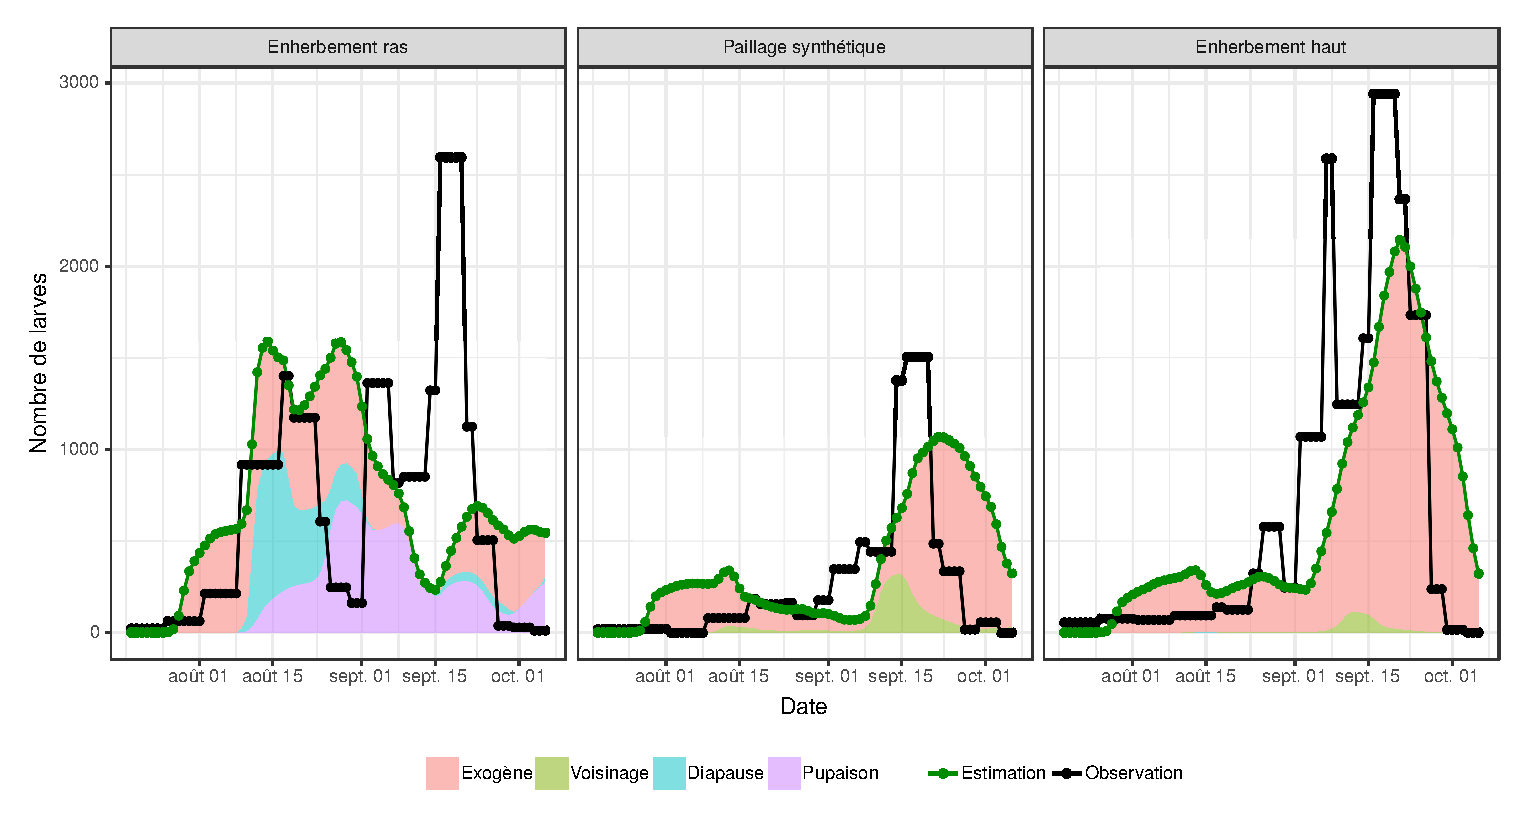
\epsfig{file = plots/full_exo.eps, scale = 0.5}
 % full_exo.eps: 2987x1595 px, 300dpi, 25.29x13.50 cm, bb=0 0 717 383
\end{figure}

Bloc 2
 \begin{figure}[ht]
 \centering
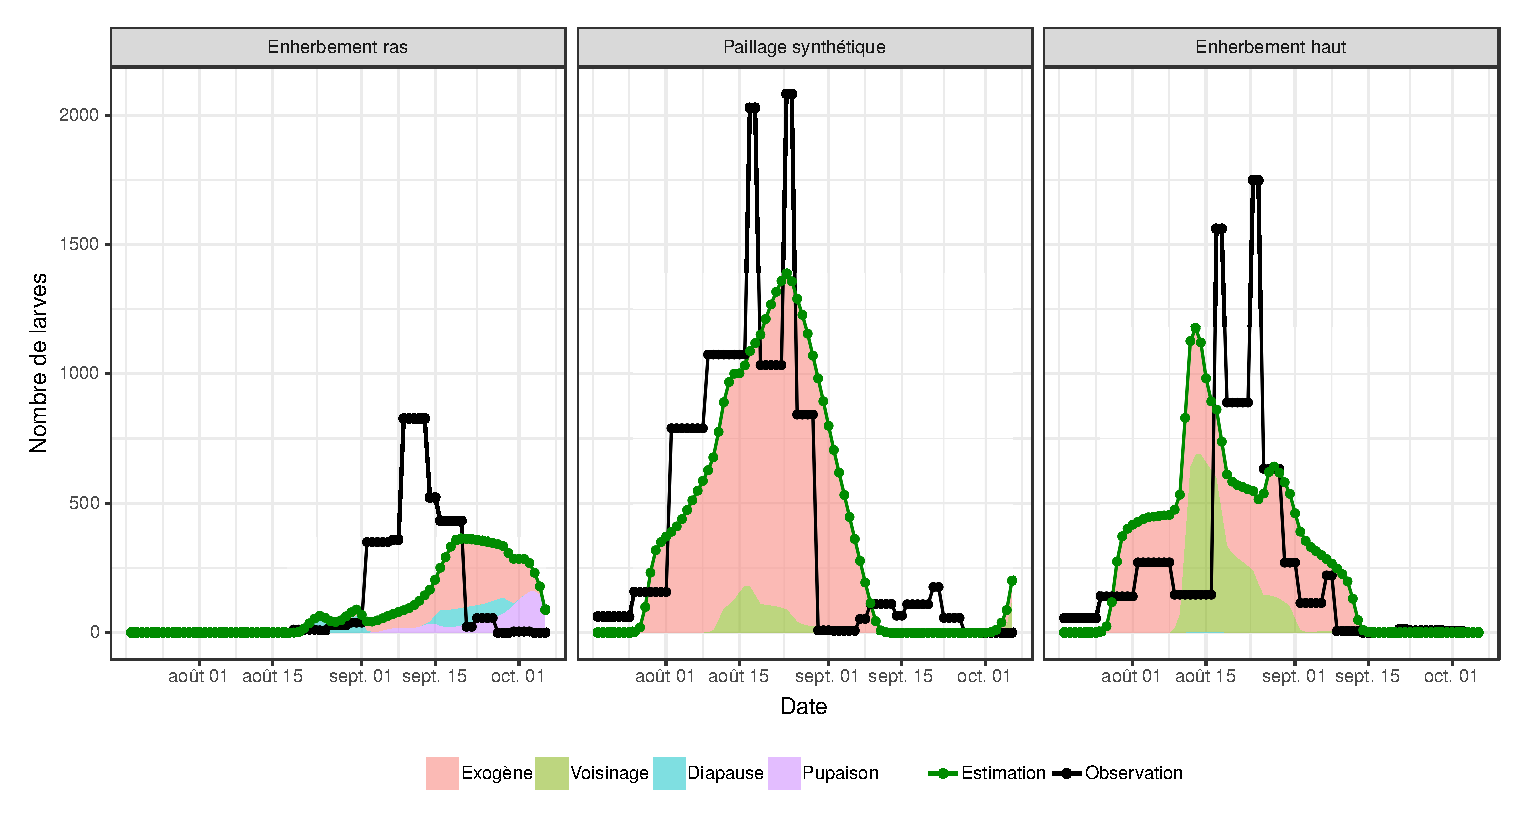
\epsfig{file = plots/1_b2.eps, scale = 0.5}
 % full_exo.eps: 2987x1595 px, 300dpi, 25.29x13.50 cm, bb=0 0 717 383
\end{figure}


 \clearpage
 \paragraph{Moins d'exogènes, moins bien ajusté}
  \begin{center}
\begin{tabular}{lllllll}
$\gamma$ & $p_m$ & $\mu_{ER}$ & $\mu_{EH}$ & $k$ & \texttt{stock} & $E_0 \mu_{\ell}$\\
0.099 & 0.334 & 0.941 & 0.893 & 12 & 12212 & 2.2
 \end{tabular}
 \end{center}
 
 Bloc 1
  \begin{figure}[ht]
 \centering
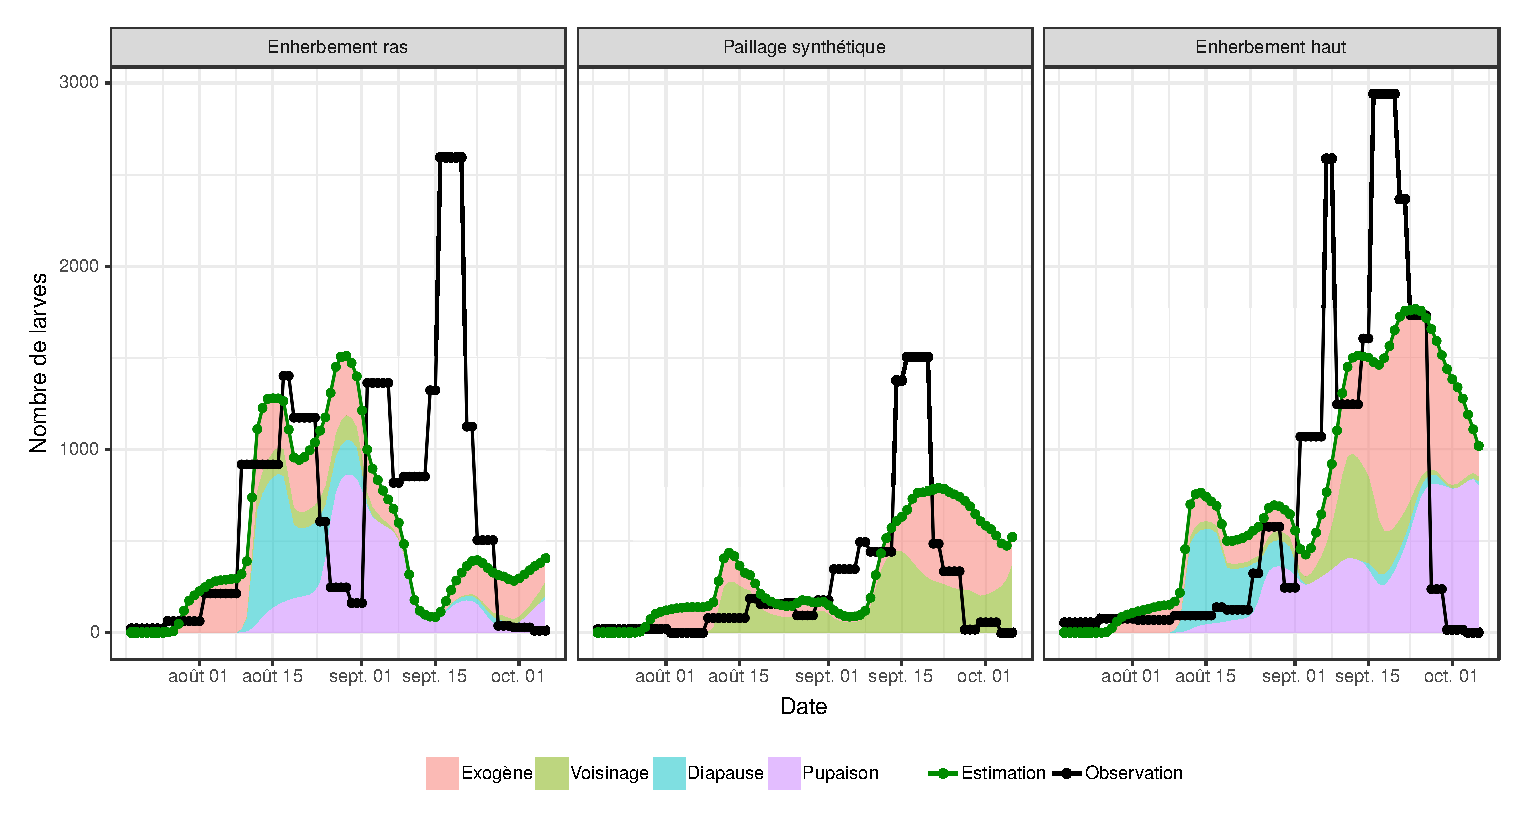
\epsfig{file = plots/2.eps, scale = 0.65}
 % full_exo.eps: 2987x1595 px, 300dpi, 25.29x13.50 cm, bb=0 0 717 383
\end{figure}
 
 Bloc 2
  \begin{figure}[ht]
 \centering
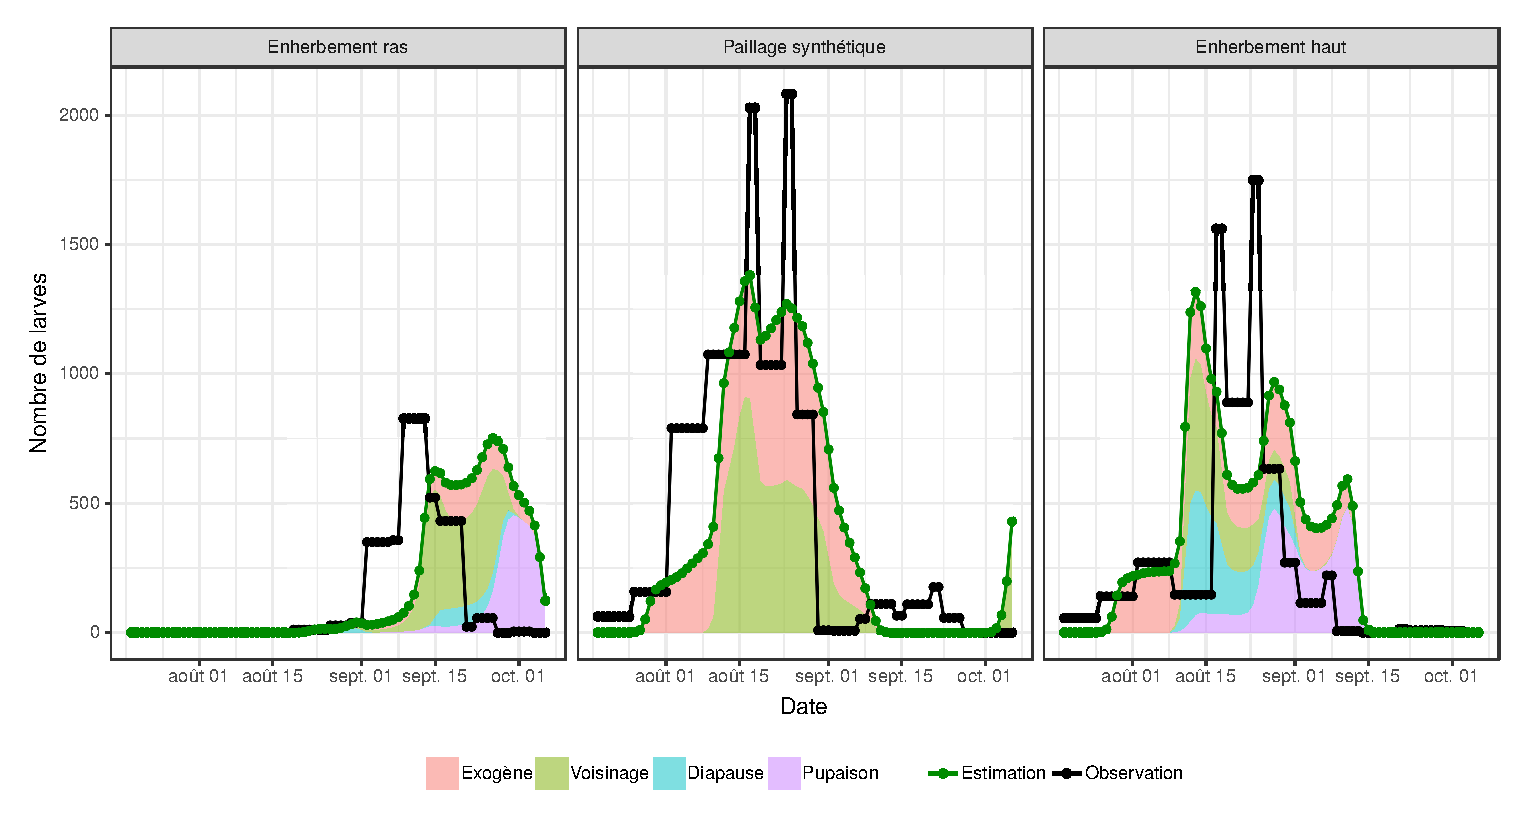
\epsfig{file = plots/2_b2.eps, scale = 0.65}
 % full_exo.eps: 2987x1595 px, 300dpi, 25.29x13.50 cm, bb=0 0 717 383
\end{figure}
 
 
 \clearpage
 \paragraph{Arrivée d'éxogènes constantes (30 femelles par jour par sous-bloc)}
   \begin{center}
\begin{tabular}{llllll}
 $p_m$ & $\mu_{ER}$ & $\mu_{EH}$ & $k$ & \texttt{stock} & $E_0 \mu_{\ell}$\\
 0.6 & 0.994 & 0.010 & 23& 10915 & 4.23
 \end{tabular}
 \end{center}
 
 Bloc 1
  \begin{figure}[ht]
 \centering
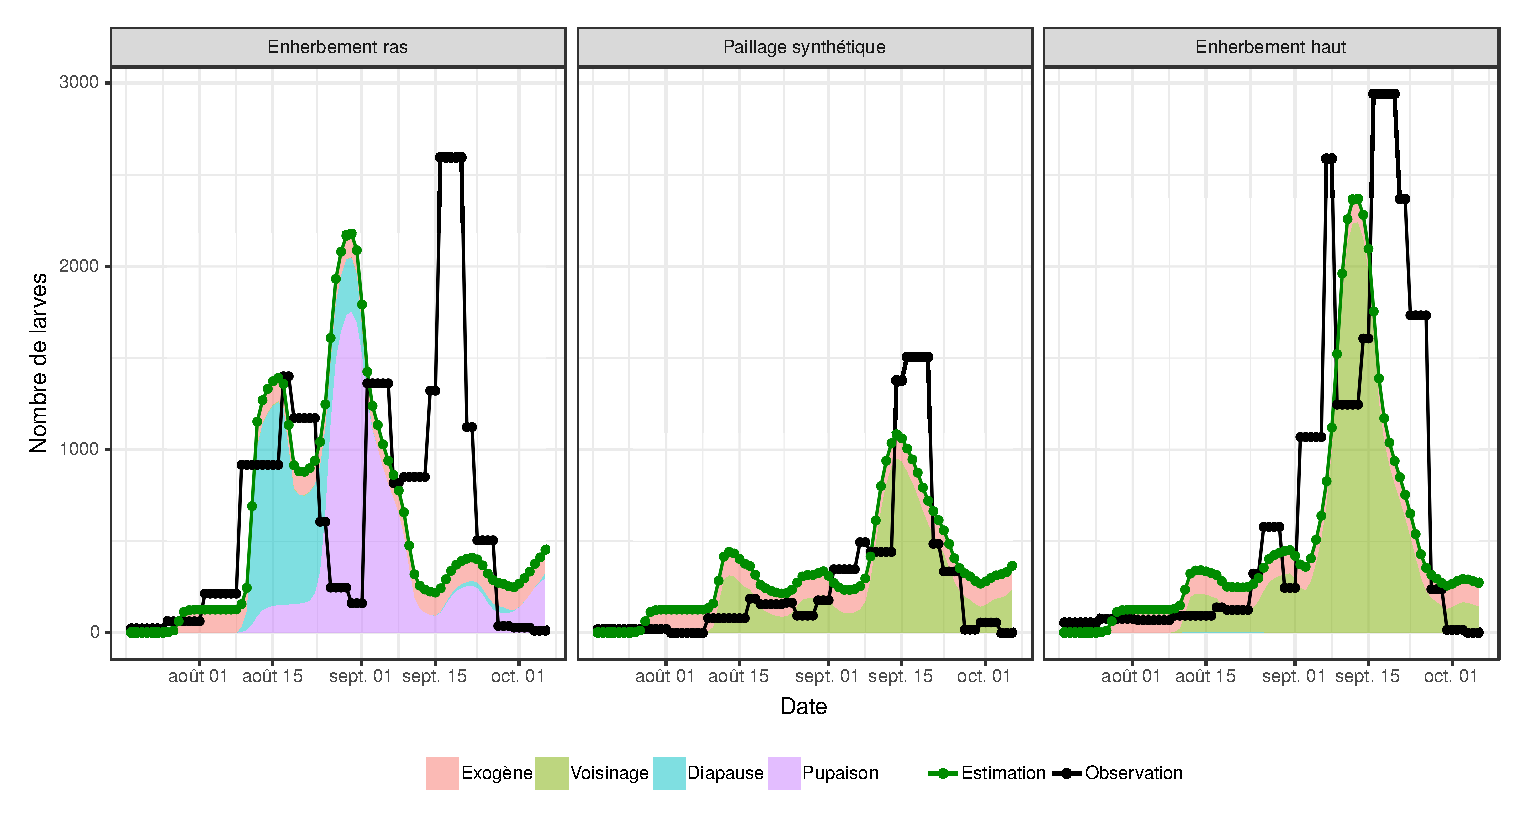
\epsfig{file = plots/3.eps, scale = 0.65}
 % full_exo.eps: 2987x1595 px, 300dpi, 25.29x13.50 cm, bb=0 0 717 383
\end{figure}
 
 Bloc 2
  \begin{figure}[ht]
 \centering
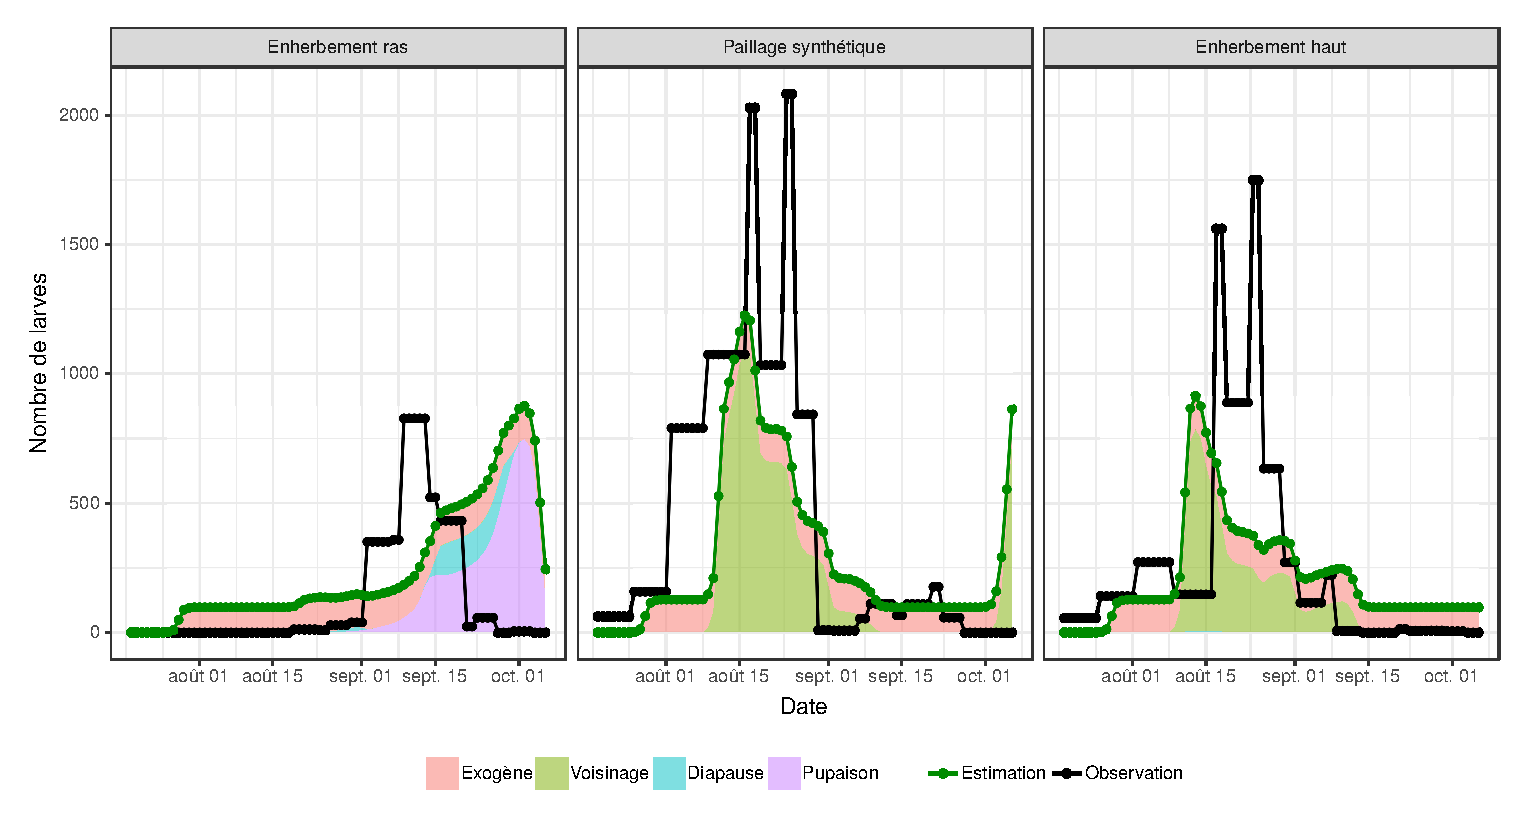
\epsfig{file = plots/3_b2.eps, scale = 0.65}
 % full_exo.eps: 2987x1595 px, 300dpi, 25.29x13.50 cm, bb=0 0 717 383
\end{figure}
 
 
\clearpage
 \paragraph{Bon ajustement basé sur les échanges}
   \begin{center}
\begin{tabular}{lllllll}
$\gamma$ & $p_m$ & $\mu_{ER}$ & $\mu_{EH}$ & $k$ & \texttt{stock} & $E_0 \mu_{\ell}$\\
0.04 & 0.6 & 0.994 & 0.010 & 23& 10915 & 4.23
 \end{tabular}
 \end{center}
 
 Bloc 1
  \begin{figure}[ht]
 \centering
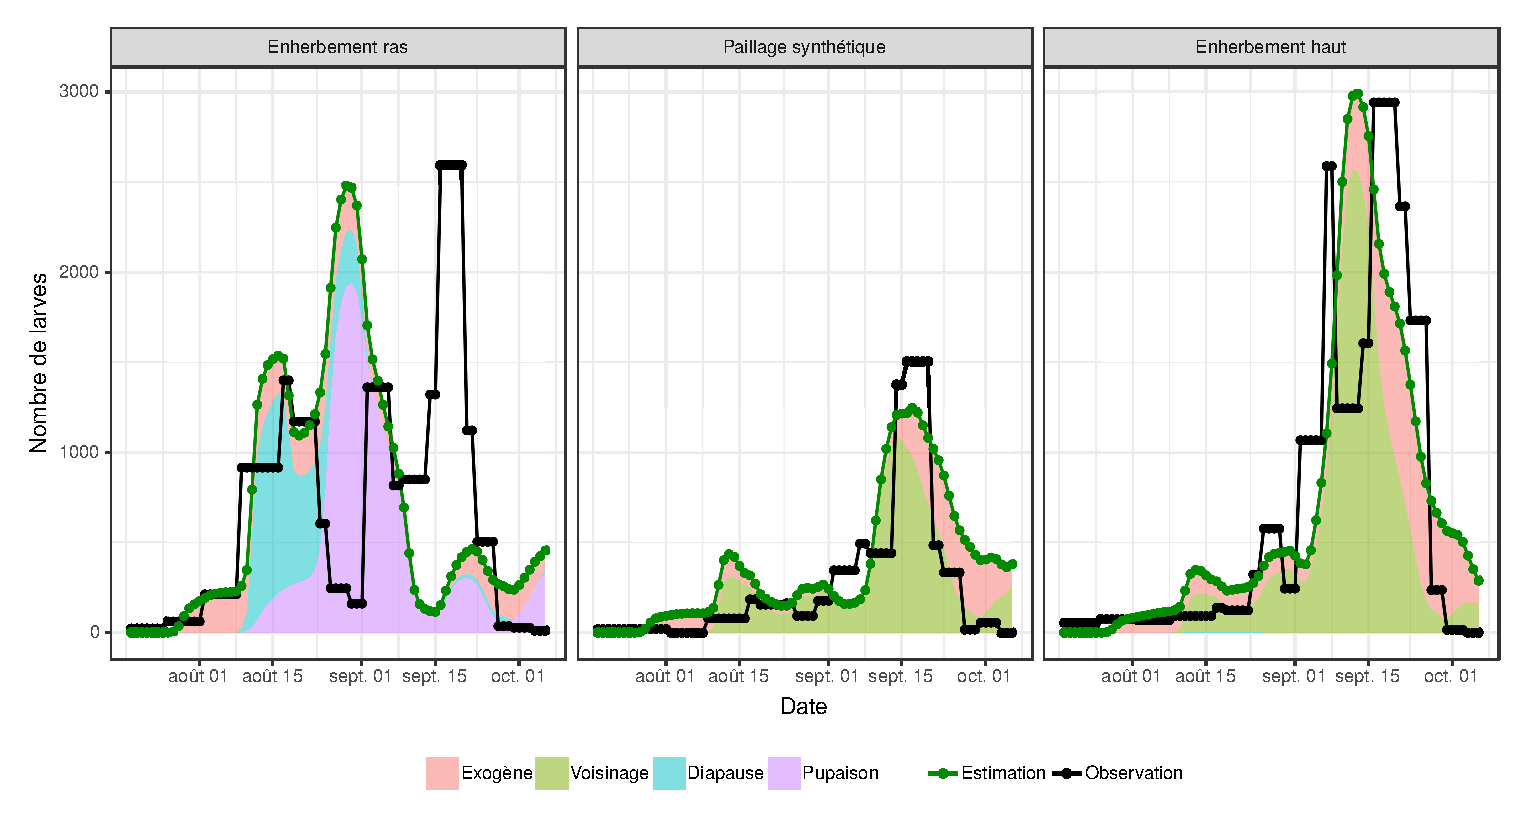
\epsfig{file = plots/5.eps, scale = 0.65}
 % full_exo.eps: 2987x1595 px, 300dpi, 25.29x13.50 cm, bb=0 0 717 383
\end{figure}
 
 Bloc 2
  \begin{figure}[ht]
 \centering
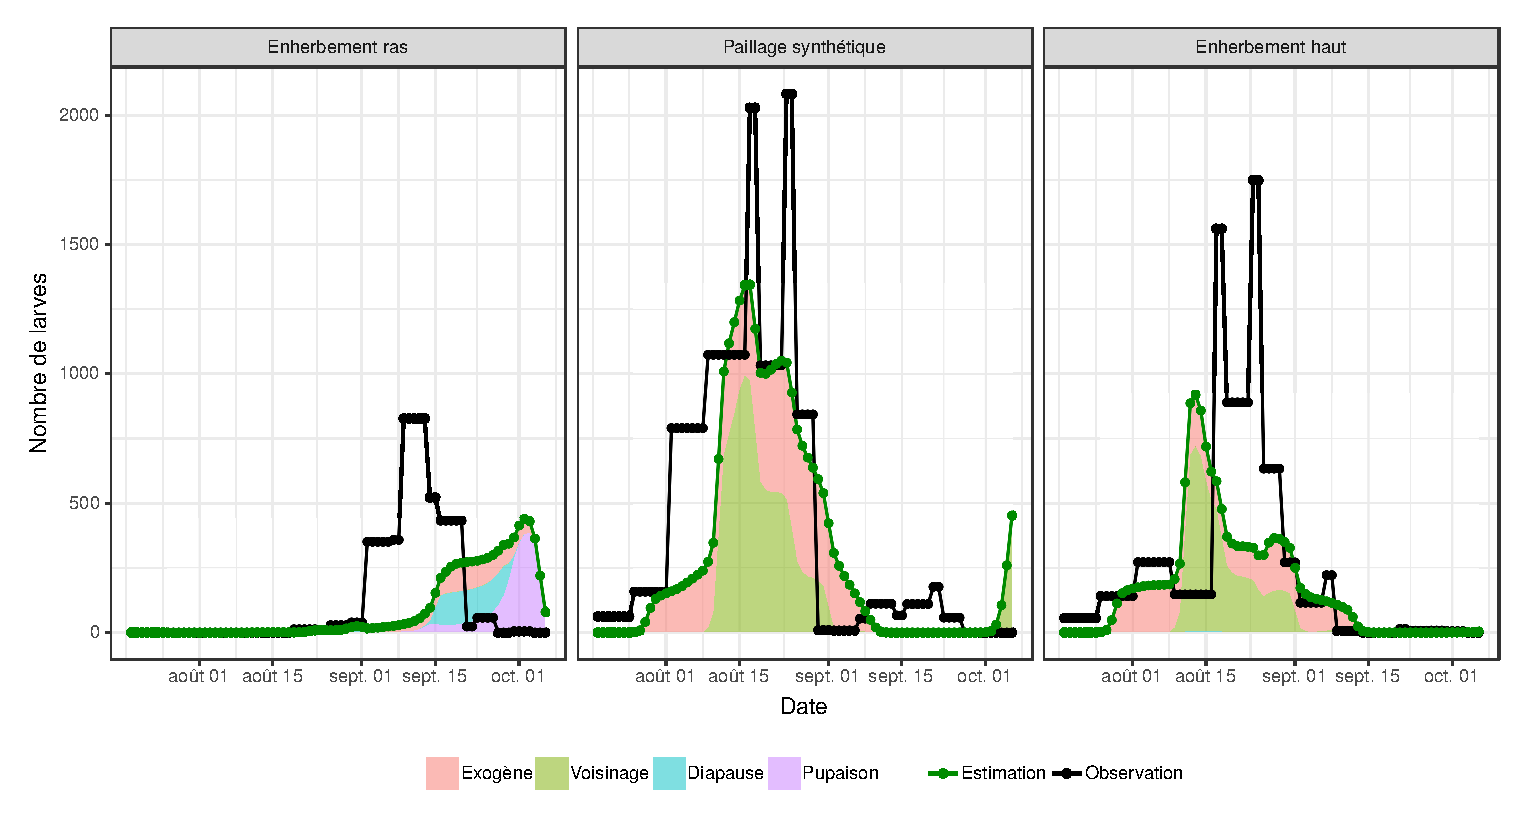
\epsfig{file = plots/5_b2.eps, scale = 0.65}
 % full_exo.eps: 2987x1595 px, 300dpi, 25.29x13.50 cm, bb=0 0 717 383
\end{figure}
 
 
 \clearpage
  \paragraph{Introduction d'un paramètre de saisonnalité sur femelles}
   \begin{center}
\begin{tabular}{llllllll}
$\gamma$ & $p_m$ & $\mu_{ER}$ & $\mu_{EH}$ & $k$ & \texttt{stock} & $E_0 \mu_{\ell}$ & \texttt{end}\\
0.1 & 0.104 & 1 & 0.999 & 58 & 10900 & 2.4 & 0.103
 \end{tabular}
 \end{center}
 
 Bloc 1
  \begin{figure}[ht]
 \centering
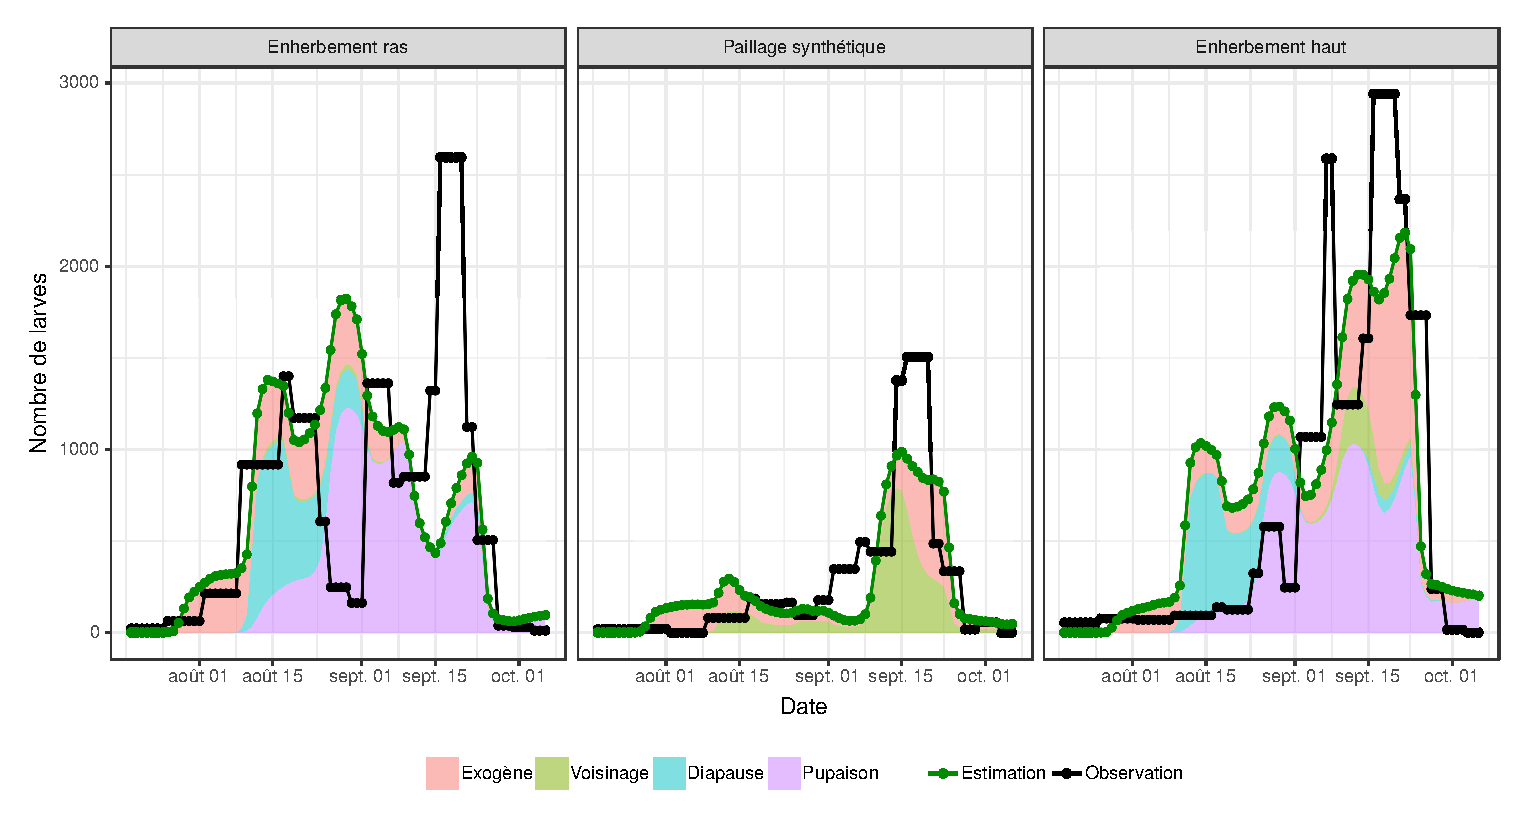
\epsfig{file = plots/4.eps, scale = 0.65}
 % full_exo.eps: 2987x1595 px, 300dpi, 25.29x13.50 cm, bb=0 0 717 383
\end{figure}
 
 Bloc 2
  \begin{figure}[ht]
 \centering
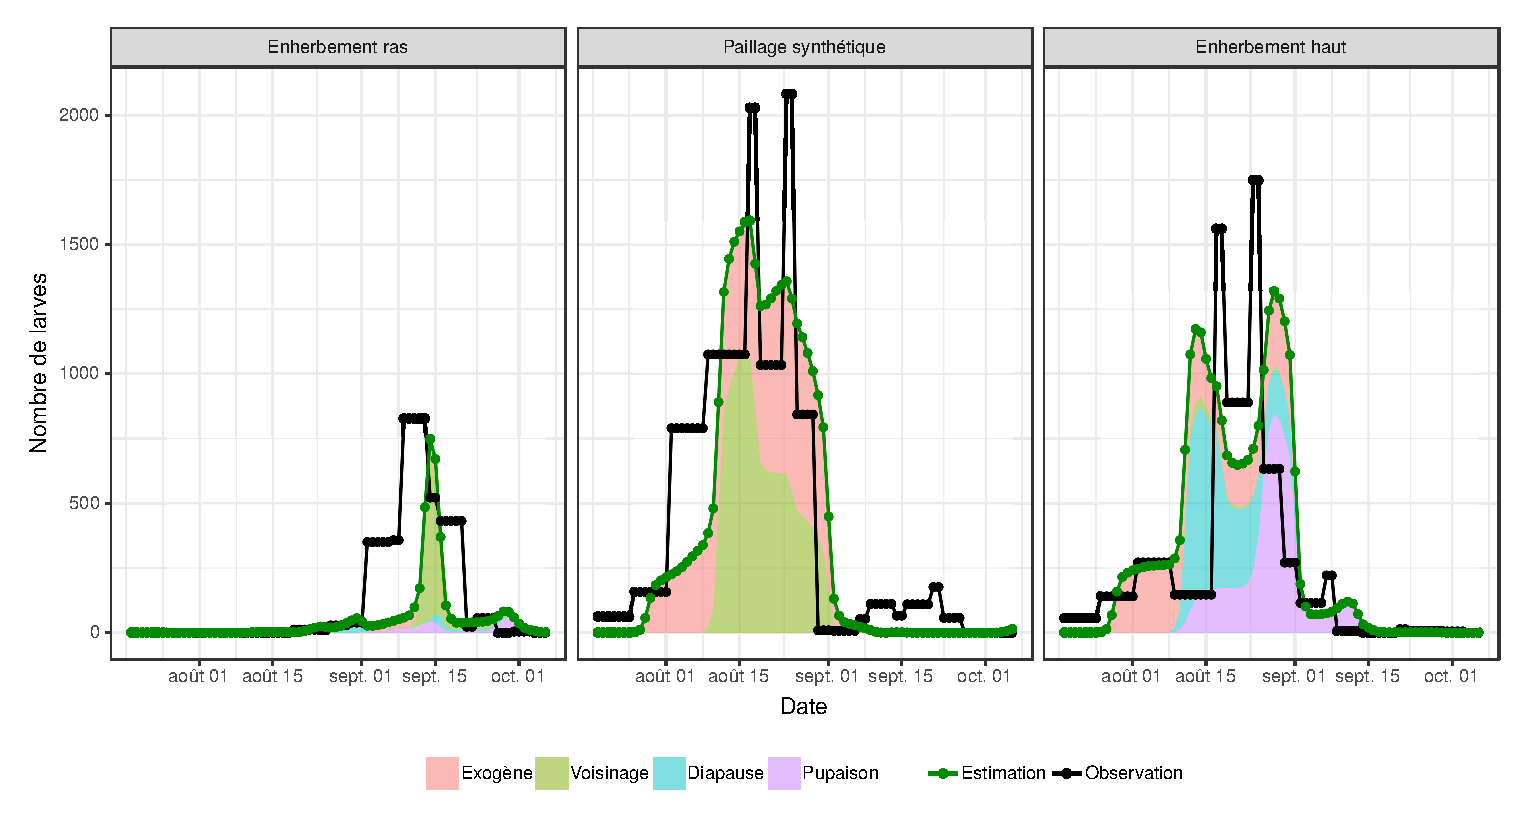
\epsfig{file = plots/4_b2.eps, scale = 0.65}
 % full_exo.eps: 2987x1595 px, 300dpi, 25.29x13.50 cm, bb=0 0 717 383
\end{figure}
 
 
 \clearpage
  \paragraph{Saisonnalité sur femelles, sans diapause}
   \begin{center}
\begin{tabular}{lllllll}
$\gamma$ & $p_m$ & $\mu_{ER}$ & $\mu_{EH}$ & $k$ & $E_0 \mu_{\ell}$ & \texttt{end}\\
0.028 & 0.051 & 0.926 & 0.930 & 72 & 6.184 & 0.018
 \end{tabular}
 \end{center}
 
 Bloc 1
  \begin{figure}[ht]
 \centering
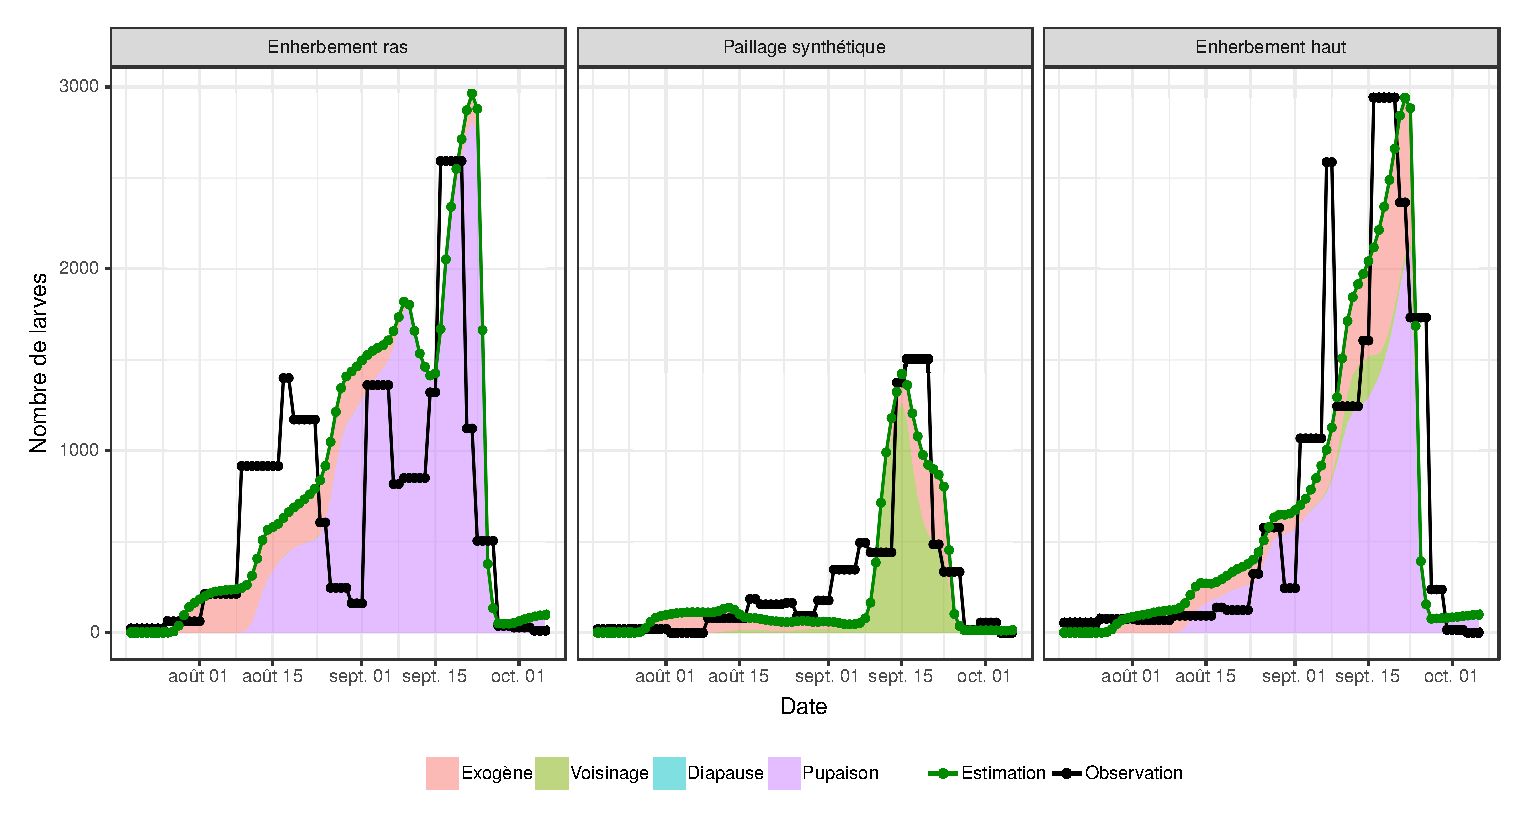
\epsfig{file = plots/6.eps, scale = 0.65}
 % full_exo.eps: 2987x1595 px, 300dpi, 25.29x13.50 cm, bb=0 0 717 383
\end{figure}

Bloc 2
  \begin{figure}[ht]
 \centering
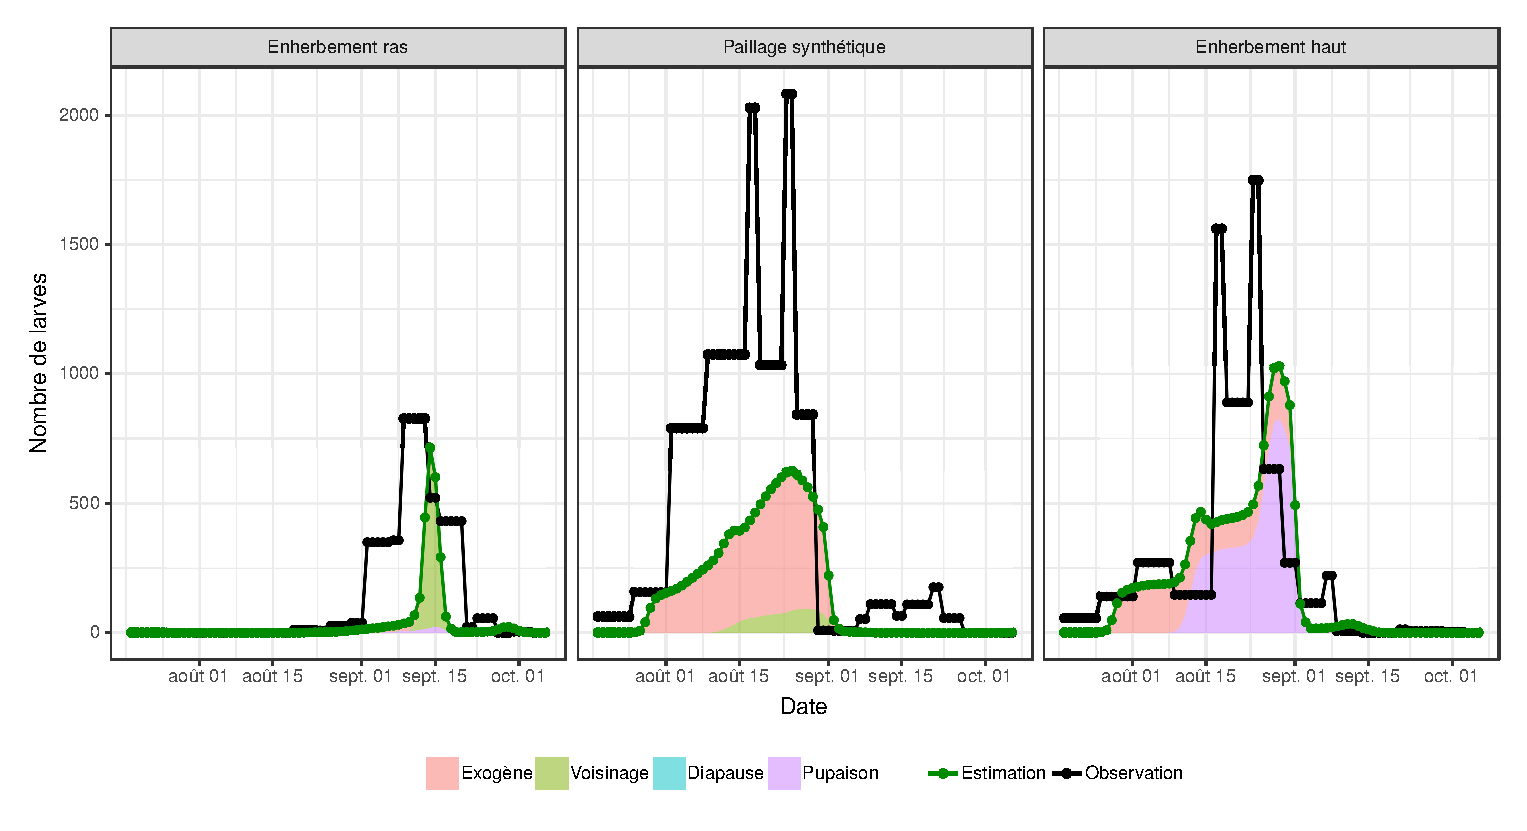
\epsfig{file = plots/6_b2.eps, scale = 0.65}
 % full_exo.eps: 2987x1595 px, 300dpi, 25.29x13.50 cm, bb=0 0 717 383
\end{figure}

 \clearpage
  \paragraph{Introduction d'un paramètre de saisonnalité sur les inflorescences}
   \begin{center}
\begin{tabular}{llllllll}
$\gamma$ & $p_m$ & $\mu_{ER}$ & $\mu_{EH}$ & $k$ & \texttt{stock} & $E_0 \mu_{\ell}$ & \texttt{end}\\
0.054 & 0.613 & 0.948 & 0.183 & 96 & 10945 & 3.891 & 0.000
 \end{tabular}
 \end{center}
 
 Bloc 1
  \begin{figure}[ht]
 \centering
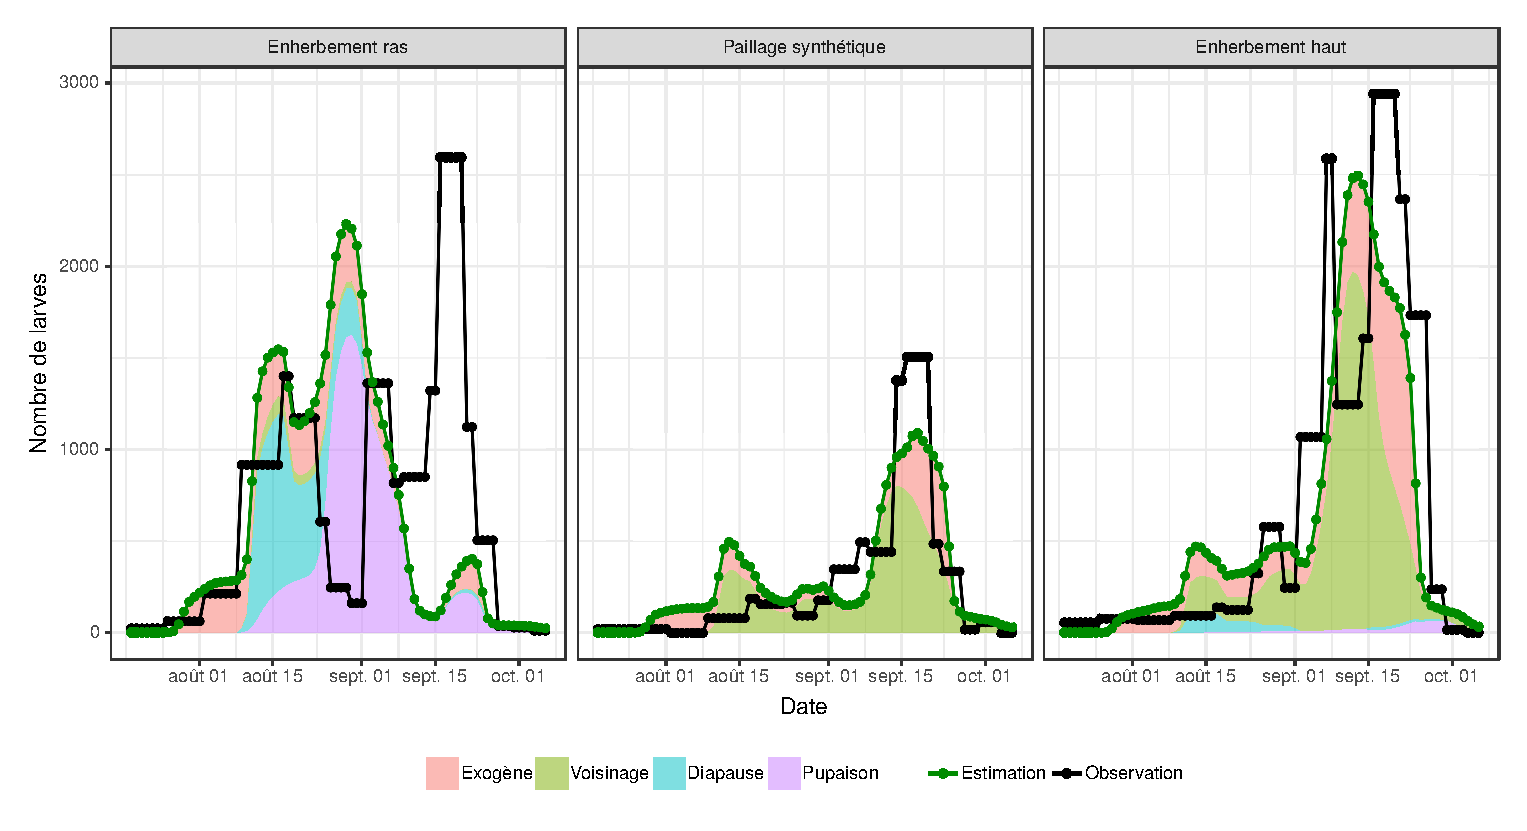
\epsfig{file = plots/7.eps, scale = 0.65}
 % full_exo.eps: 2987x1595 px, 300dpi, 25.29x13.50 cm, bb=0 0 717 383
\end{figure}

Bloc 2
  \begin{figure}[ht]
 \centering
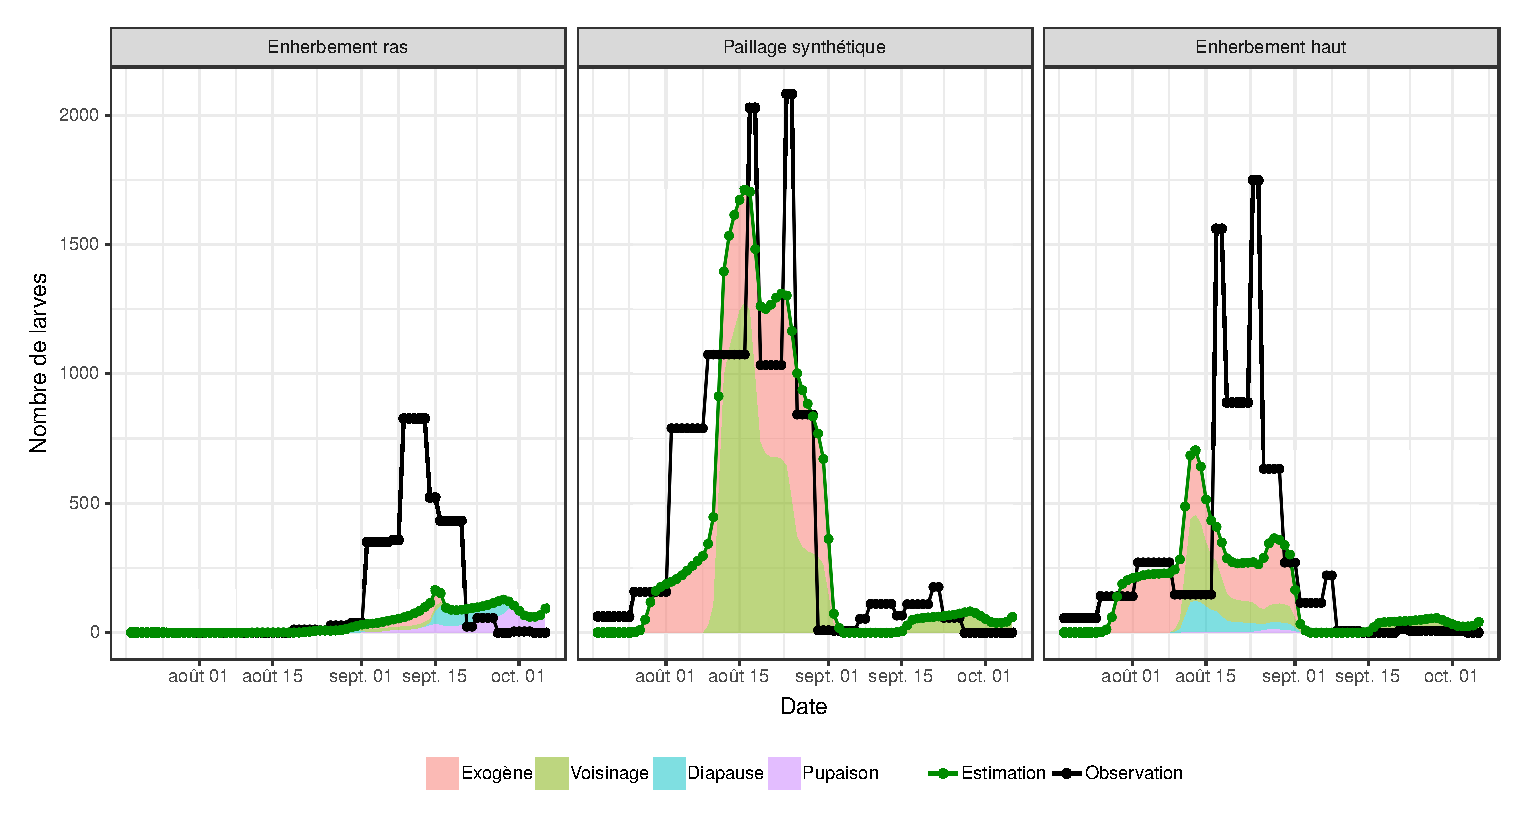
\epsfig{file = plots/7_b2.eps, scale = 0.65}
 % full_exo.eps: 2987x1595 px, 300dpi, 25.29x13.50 cm, bb=0 0 717 383
\end{figure}
 

 \clearpage
  \paragraph{Saisonnalité sur les inflorescences, sans diapause}
   \begin{center}
\begin{tabular}{lllllll}
$\gamma$ & $p_m$ & $\mu_{ER}$ & $\mu_{EH}$ & $k$ & $E_0 \mu_{\ell}$ & \texttt{end}\\
0.025 & 0.059 & 0.908 & 0.928 & 12 & 6.46 & 0
\end{tabular}
 \end{center}
 
 Bloc 1
  \begin{figure}[ht]
 \centering
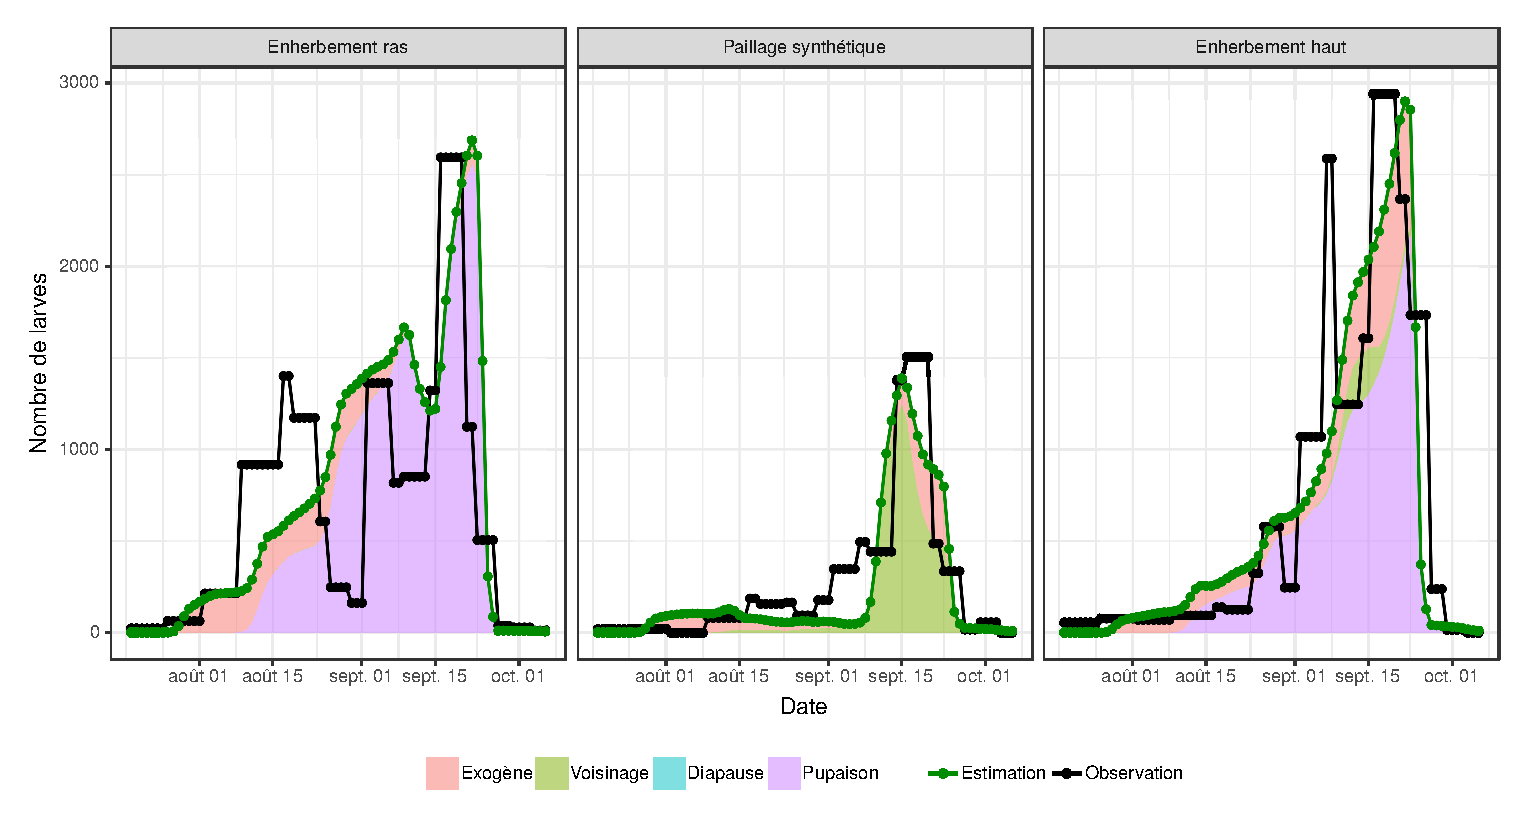
\epsfig{file = plots/8.eps, scale = 0.65}
 % full_exo.eps: 2987x1595 px, 300dpi, 25.29x13.50 cm, bb=0 0 717 383
\end{figure}
 
 Bloc 2
  \begin{figure}[ht]
 \centering
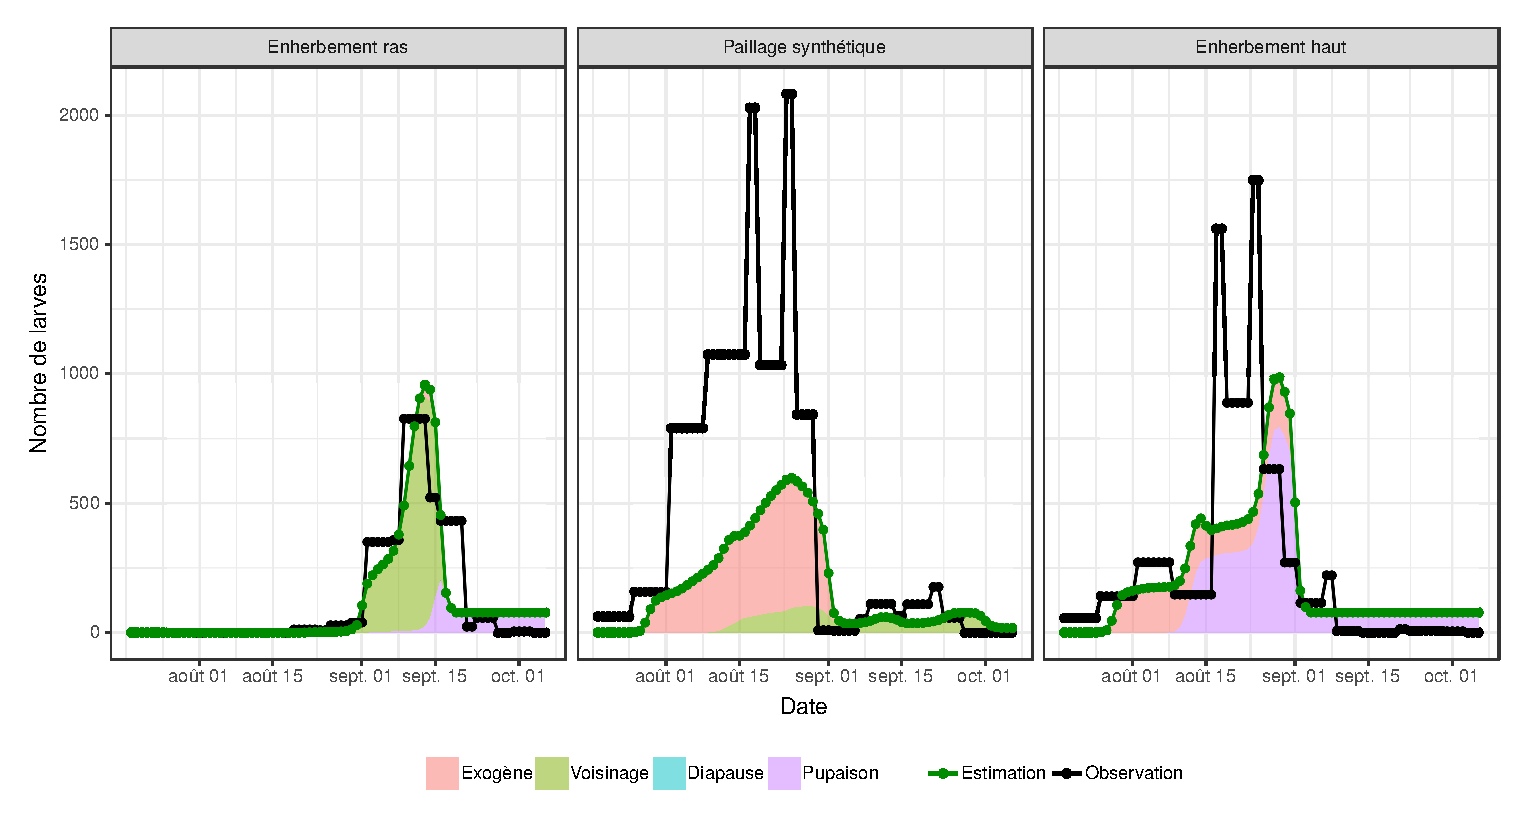
\epsfig{file = plots/8_b2.eps, scale = 0.65}
 % full_exo.eps: 2987x1595 px, 300dpi, 25.29x13.50 cm, bb=0 0 717 383
\end{figure}
 
  
 \clearpage
  \paragraph{Exogène : 30 femelles, saisonnalité : femelles}
   \begin{center}
\begin{tabular}{lllllll}
 $p_m$ & $\mu_{ER}$ & $\mu_{EH}$ & $k$ & \texttt{stock} & $E_0 \mu_{\ell}$ & \texttt{end}\\
 0.3 & 0.8 & 0.9 & 38 & 10900 & 4.497 & 0.041
\end{tabular}
 \end{center}
 
 Bloc 1
  \begin{figure}[ht]
 \centering
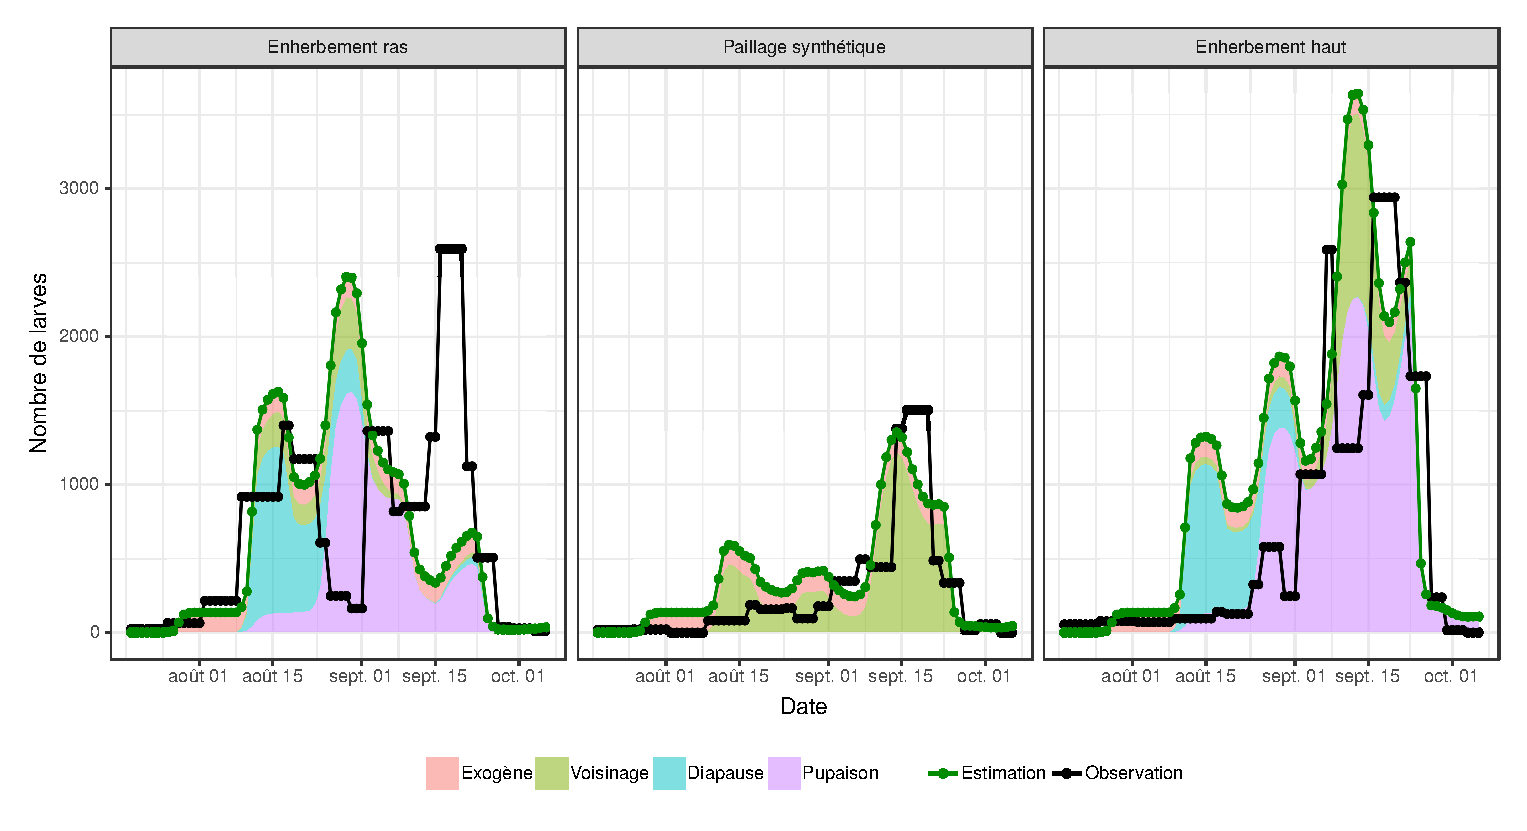
\epsfig{file = plots/9.eps, scale = 0.65}
 % full_exo.eps: 2987x1595 px, 300dpi, 25.29x13.50 cm, bb=0 0 717 383
\end{figure}

Bloc 2
  \begin{figure}[ht]
 \centering
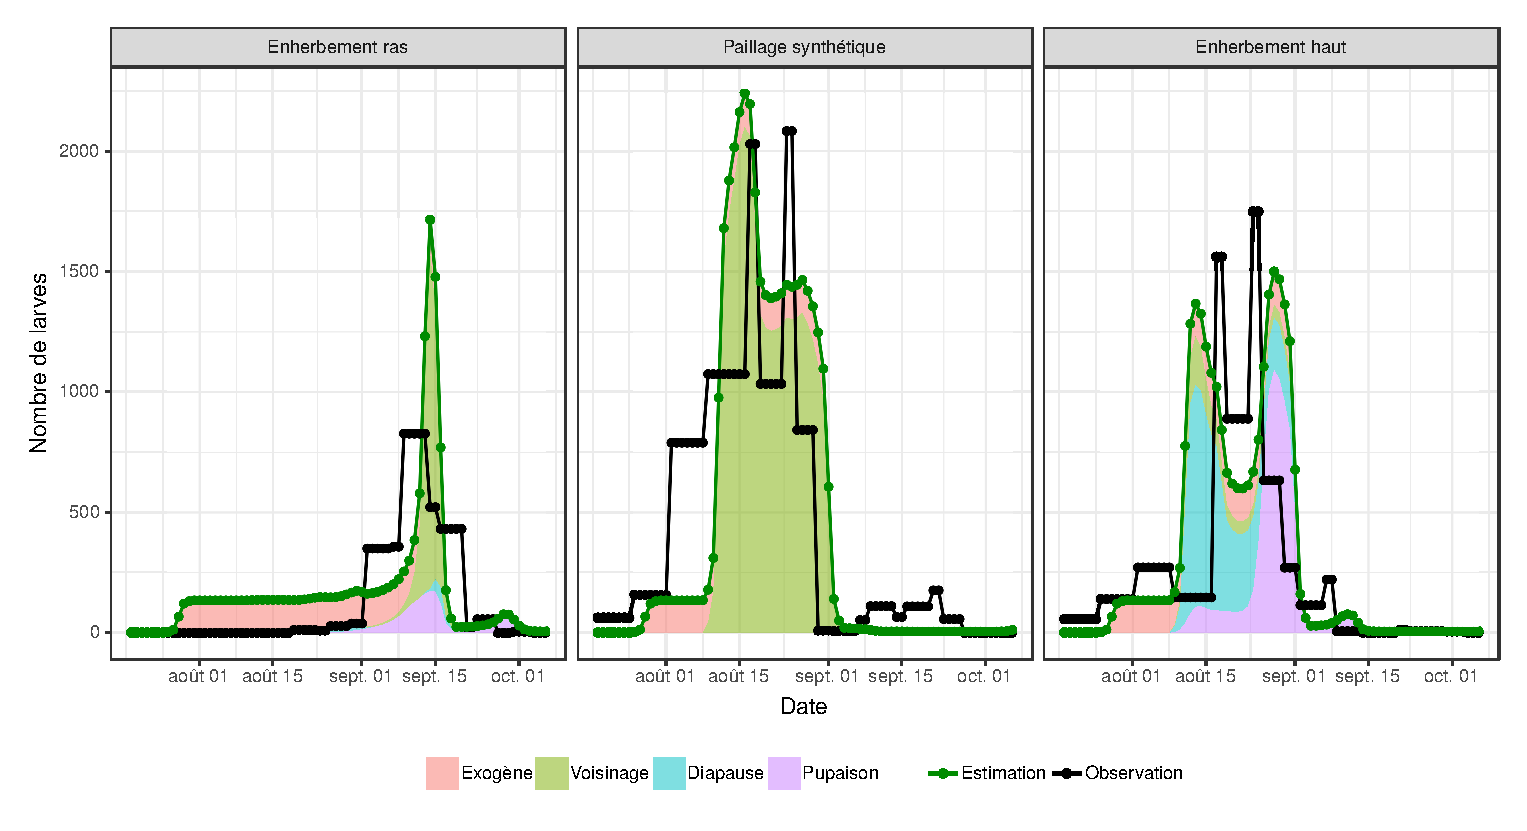
\epsfig{file = plots/9_b2.eps, scale = 0.65}
 % full_exo.eps: 2987x1595 px, 300dpi, 25.29x13.50 cm, bb=0 0 717 383
\end{figure}

 
\end{document}
